\documentclass[svgnames,13pt]{beamer}
\usepackage{ifthen}
\newboolean{UseNotes}

% ###################################### %
\newcommand{\Date}		{September 12 2012}
\newcommand{\Author}	{Frederik Mogensen}
\newcommand{\Title}		{Outsourced similarity search on metric data}
\newcommand{\subTitle}	{Mironov, Pandey, Reingold \& Vadhan}
\newcommand{\Subject}	{Multidimensional databases}
\newcommand{\Faculty}	{Computer Science}
\setboolean{UseNotes}	{true}
\newcommand{\ColorHead}	{DarkSlateGrey}
\newcommand{\ColorRest}	{darkgray}
%% Color choices on page 38 in
%% http://www.math.washington.edu/tex-archive/macros/latex/contrib/xcolor/xcolor.pdf
% ###################################### %


%% Use notes ?
\ifthenelse{\boolean{UseNotes}}
	{
		%%% Notes
		\usepackage{pgfpages}
		\setbeameroption{show notes}
		\setbeameroption{show notes on second screen=right}
		\setbeamertemplate{note page}{
		\bigskip
		\insertsubsectionnavigation{\textwidth}
		\insertnote
	}
	{
		%%% No Notes
	}
}

\usetheme{default}
\setbeamertemplate{navigation symbols}{} %gets rid of navigation symbols
\setbeamertemplate{itemize items}[circle]
\setbeamercolor{titlelike}{fg=\ColorHead}
\setbeamercolor{item}{fg=\ColorRest}
\setbeamercolor{normal text}{fg=\ColorRest}

%%% Background
\usebackgroundtemplate{
	\vbox to \paperheight{\vspace{0.4cm}
	\hspace{1.0cm}
\includegraphics[width=5cm]{img/au.png}\hfill\vfill}
}

% ------------------------------------------------------------------------------
% frametitle
% ------------------------------------------------------------------------------
\setbeamertemplate{frametitle}
{
	\begin{flushleft}
		\vspace{0.8cm}
		{\Large \textbf{\textmd{\insertframetitle}}}\\
		\vspace{-0.4cm}
		\line(1,0){100}\hfill
		\vspace{-0.6cm}
	\end{flushleft}
}

% ------------------------------------------------------------------------------
% footer
% ------------------------------------------------------------------------------
\setbeamertemplate{footline}{
	\begin{minipage}[b]{0.88\linewidth}
		\flushright{\tiny{\MakeUppercase{\Author}\\
		\vspace{-0.5cm}\MakeUppercase{\Title}}} \\
	\end{minipage}
	\hfill
	\begin{minipage}[b]{1.1\linewidth}

		\vspace{-3em}
		\hspace{\fill}\line(1,0){200}\hspace{0.2cm}\line(1,0){62}
		\vspace{0.2cm}

		\flushright{\tiny{\insertframenumber\\ \vspace{-0.5cm}\Date}}
	\end{minipage}

	\vspace{0.7cm}
}

\usepackage{beamerfontthemeprofessionalfonts}
\usepackage{graphicx}
\usepackage[english]{babel}
\usepackage[utf8]{inputenc}
\usepackage{amsmath}
\usepackage{amssymb}
\usepackage{amsthm}

\usepackage{multirow}
\usepackage{booktabs}

\begin{document}

% ------------------------------------------------------------------------------
% title
% ------------------------------------------------------------------------------

\begin{frame}[plain]
	\hfill
	\begin{minipage}[]{0.4\linewidth}
		\flushright{\tiny{\Faculty\\ \vspace{-0.2cm} \Date}}
	\end{minipage}
	\\
	\vspace{1.cm}
	\huge{\MakeUppercase{\Title}} \\
	\vspace{0.2cm}\small{\subTitle}
	\vspace{0.5cm}
	\hfill
	\linethickness{3pt}
	\flushright{
		\vspace{-1.0cm}
		\line(1,0){230}
		\vspace{0.2cm}
		\hfill
	}
	\linethickness{1pt}

	\begin{minipage}[b]{\linewidth}
		\Large{\Author} \hfill
	\end{minipage}

	\vfill
	\vspace{2cm}
	\begin{minipage}[b]{1.0\linewidth}
		\hfill \LARGE{\MakeUppercase{\Subject}}
	\end{minipage}
\end{frame}

% ------------------------------------------------------------------------------
% introduction
% ------------------------------------------------------------------------------

    \begin{frame}[t]
	\frametitle{Headline - Very Serious}
	One item
	\begin{itemize}
		\item Here it is.
	\end{itemize}
	\pause
	\vspace{0.5cm}
	Two items
	\begin{itemize}
		\item Item 1. \pause
		\item Item 2.
		\item Item 3.
	\end{itemize}
	\note[item] {Not actually serious}
	\note[item] {
	Venn Diagrams
	\\
		\begin{figure}[h]
			\centering
			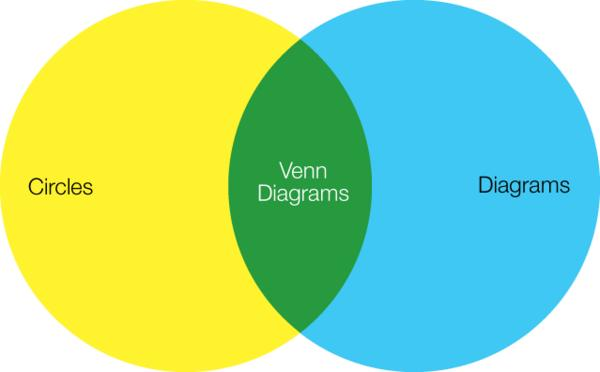
\includegraphics[height=\textheight/2]{img/venndiagram.jpeg}
			\label{fig:venndiagram-meta}
		\end{figure}
	}
\end{frame}

\begin{frame}[t]
	\frametitle{Range query searching}
	\begin{block}{S1. [Search subtrees.]}
		 Check each entry $E$ to determine whether the MBR overlaps $q$.
		 For all overlapping entries, invoke \emph{Search} on the tree whose
		 root is pointed to by $E.p$
	\end{block}

	\begin{block}{S2. [Search leaf node.]}
		Check all entries $E$ to determine whether the MBR overlaps $q$.
		If so, $E$ is a qualifying record
	\end{block}
\end{frame}



\end{document}
